Following methods are used to implement Shor's algorithm to factor an integer.
\section{Hardware}
Since Shor's algorithm is a quantum algorithm, a quantum computer is necessary to implement an example of the factorization of an integer. Fortunately, IBM Quantum allows some of its prototype quantum computers to be used by the public for research and other applications via its interface platform IBM Quantum Experience(ibmq).\cite{devitt2016} IBM Quantum experience is a cloud-based platform that allows users to send quantum algorithm or program as a job for it to be executed on the quantum computer at IBM. Quantum computers at IBM are housed with superconducting qubits composed of coupled Josephson junction, also known as transmon qubits. \cite{fisher_2009}. IBM classify their quantum computer into open and premium system.\cite{ibmq_backends} They allow the use of open quantum systems via backends at IBM Quantum for enthusiasts and researchers. At the time of writing, there are six open quantum systems available as given in the table below.
\begin{table}[h]
\begin{tabular}{|l|l|lll}
\cline{1-2}
Name                & Qubits    \\ \cline{1-2}
ibmq\_santiago      & 5          \\ \cline{1-2}
ibmq\_athens        & 5         \\ \cline{1-2}
ibmq\_16\_melbourne & 15        \\ \cline{1-2}
ibmq\_armonk         & 1        \\ \cline{1-2}

\end{tabular}
 \caption{Open Quantum systems at IBM available to public}
 \label{tab: Open Quantum systems at IBM available to public}
\end{table}

In this study, the program or circuit for Shor's algorithm is executed on a simulator and a quantum so that comparisons can be made. Following devices were used to execute the circuit:\cite{ibmq_backends}
\begin{itemize}
    \item $ibmq\_qasm\_simulator$
    \item $ibmq\_16\_melbourne$
\end{itemize}

\subsection{\textbf{$ibmq\_qasm\_simulator$}}
$ibmq\_qasm\_simulator$ is a cloud quantum simulator based at IBM quantum. It is a high-performance simulator that executes a quantum circuit written on QASM( Quantum Assembly Language). As the name suggests this simulator is not based on the quantum behavior of material but on the mathematical formulation of quantum computation. Hence they produce error-free outputs at the expense of an increase in complexity. The basic gates it uses are "U1, U2, U3, U, P, R, RX, RY, RZ, ID, X, Y, Z, H, S, SDG, SX, T, TDG, SWAP, CX, CY, CZ, CSX, CP, CU1, CU2, CU3, RXX, RYY, RZZ, RZX, CCX, CSWAP, MCX, MCY, MCZ, MCSX, MCP, MCU1, MCU2, MCU3, MCRX, MCRY, MCRZ, MCR, MCSWAP, UNITARY, DIAGONAL, MULTIPLEXER, INITIALIZE, KRAUS, ROERROR, DELAY"\cite{ibm_quantum_experience}. The version of qasm simulator used for the study is 0.1.547. 

$ibmq\_qasm\_simulator$ is used for the study rather than a local simulator to maintain consistency of output measurements in term of randomness or correctness of the output

\subsection{\textbf{$ibmq\_16\_melbourne$}}
'$ibmq\_16\_melbourne$' quantum system was used for the implementation because it was the only public system with enough qubits to run our circuit.
$ibmq\_16\_melbourne$ is a 15 qubits quantum system with quantum volume 8. It uses CX, ID, RZ, SX, and X as a basic set of gates with an average CNOT error: 0.03348 and an average readout error: 0.07161.\cite{ibm_quantum_experience} In a physical system, a coupling map is used to select a set of required qubits with the least CNOT error between all qubits. The coupling map of $ibmq\_16\_melbourne$ is as shown in figure(\ref{fig: coupling map_melbourne}).
\begin{figure}[H]
    \centering
    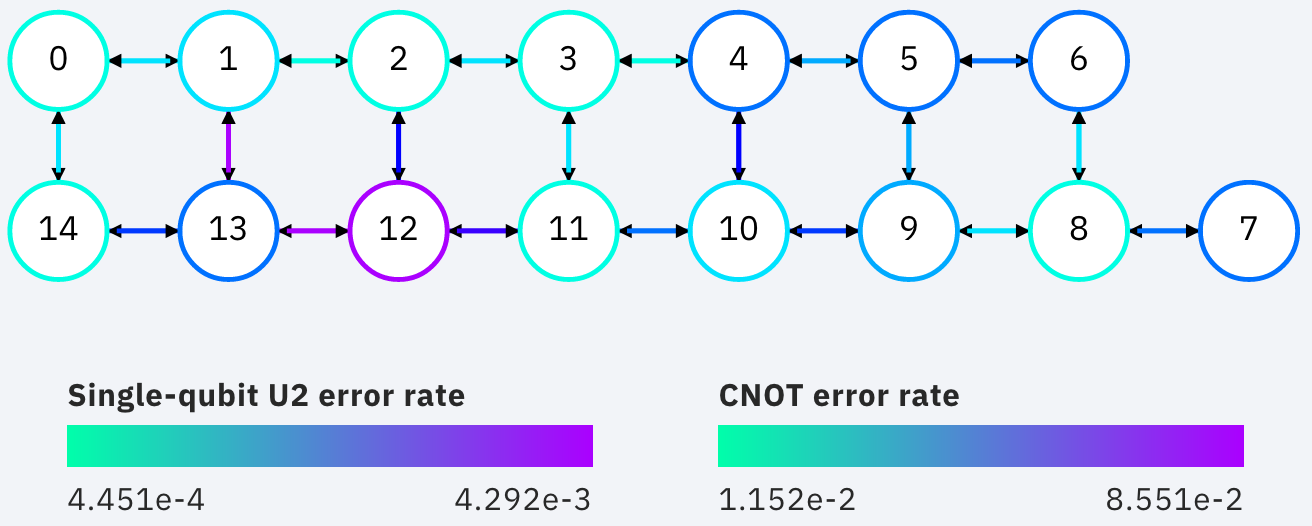
\includegraphics[width = \linewidth]{figures/coupling map_melbourne.png}
  \caption{Topology diagram and coupling map of $ibmq\_16\_melbourne$}
  \label{fig: coupling map_melbourne}
\end{figure}
The figure shows the different single-qubit error for different qubits and different CNOT gate errors for each coupling. The selection of qubits to use for the execution of circuit should be done so as to reduce the error in the circuit. Implementation of the circuit in this study requires 6 qubits for execution.Hence, qubits 0,1,2,3,13,14 were chosen for execution. 

\section{Software}
Python programming language, primarily one of its packages: QISKIT was used for our study and jupyter notebook was used as the text editor. QISKIT is an open-source software development kit that allows designing and run quantum circuits and working with quantum algorithms.\cite{qiskit_org} It has local simulators prepacked with it to run circuits. Also, it creates an interface between a local computer with IBM quantum to run on quantum systems or simulators provided by IBM. QISKIT has four main components: $Terra$, $Ignis$, $Aqua$, and $Aer$ based on their purpose.\cite{qiskit_org_documentation} $Terra$ deals with the foundation of quantum programs like quantum circuits, gate control, pulse control, and others. $Ignis$ deals with errors and noises in the system and error correction. $Aqua$ aims at the application of the quantum system for applications like optimization, chemistry. $Aer$ includes high-performance simulators emulators.

QISKIT has a feature for visualization of circuits and outputs or results. Visualization of circuits makes the understanding of workings of circuit at hardware level. Result visualization helps in better representation and faster understanding. It has built-in visualization tools to generate useful plots like histograms, Bloch sphere, qsphere of the results.

The version of QISKIT we worked on is
\\$\{
    'qiskit-terra': '0.16.2'$,\\
    $'qiskit-aer': '0.7.3',$\\
    $'qiskit-ignis': '0.5.1',$\\
    $'qiskit-ibmq-provider': '0.11.1',$\\
    $'qiskit-aqua': '0.8.1',$\\
    $'qiskit': '0.23.3'
 \}$

\section{Circuit Design}
Due to the limitation of qubits and depth of circuit, we implement a simplified compiled version of Shor's algorithm to factor a small number I=15 with base z=2 for \acrshort{MEF}. The simplified complied version of the algorithm is inspired by a paper by \cite{geller2013factoring}. This paper suggests a low depth circuit with less number of qubits for implementation of the algorithm for composite integers composed of Fermat primes\footnote{Fermat's prime are prime numbers in the form $2^{2n}$, for some integer 'n'}. However, this algorithm requires pre-knowing the order of the required \acrlong{MEF}. 

In the algorithm itself, the most difficult task: modular exponentiation is compiled into a set of few gates. For our case, the MEF gives a set $\{1,2,3,4\}$. Their binary equivalence can be encoded in two qubits. hence we set the period register of two qubits. For the input register, we set the number of qubits given by the equation: $n = \lfloor log_2(15)\rfloor = 4$. To store the output, we add a 4 qubit classical register. First, Hadamard gates are added to the input register to create superposition. As for MEF, two C-NOT gates CNOT($IQ_1, PQ_1$) and CNOT($IQ_2, PQ_2$), where $IQ_1$ , $IQ_2$ are qubits of input register in increasing significance and $ PQ_1$ , $ PQ_2$ are qubits of the period register in increasing significance. Finally, the Quantum Fourier transform is applied to the input register. At last. the input register(IQ) is measured and stored in classical register. The circuit diagram for it is as shown in the figure below.

\begin{figure}[H]
    \centering
    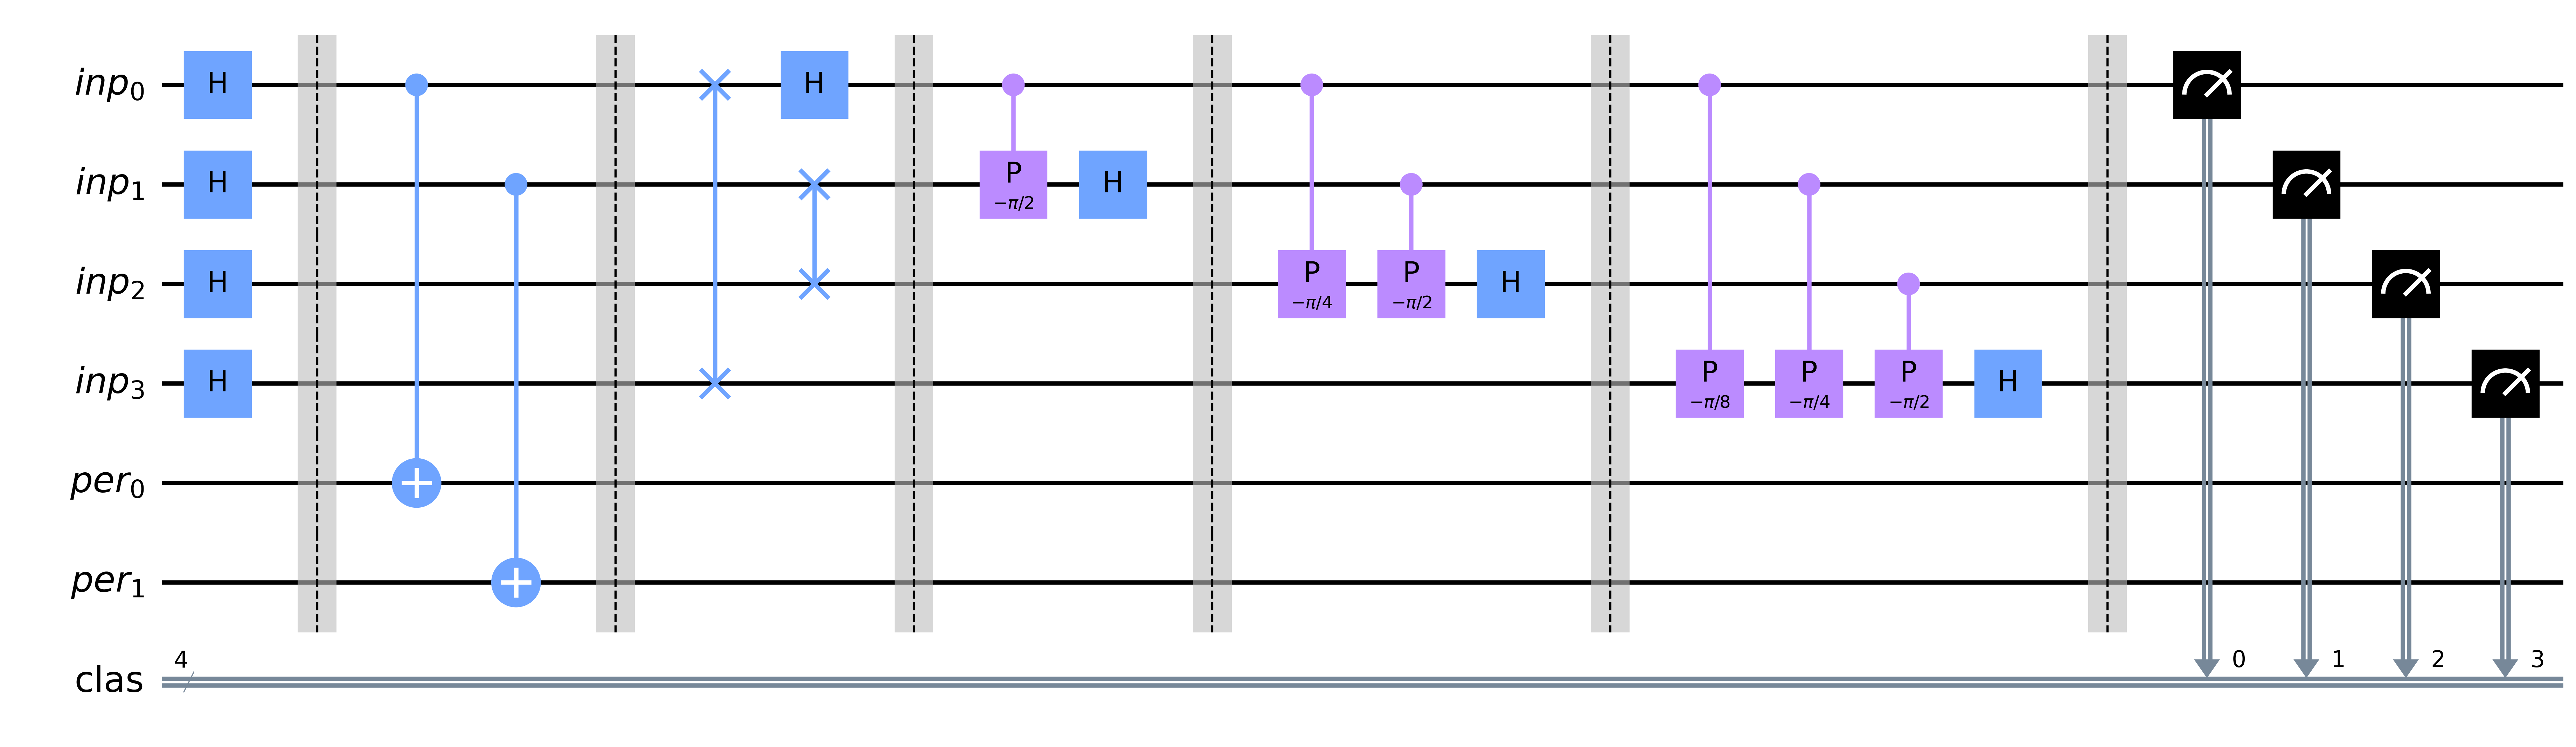
\includegraphics[width = \linewidth]{figures/shorfor15_2.png}
  \caption{Circuit Diagram for implementation of compiled shor's algorithm}
  \label{fig: Shor compiled circuit for fermat's prime}
\end{figure}

\section{Circuit Execution}
The circuit designed was then executed on a simulator and quantum computer. In both the systems, the circuit takes the following 6 sets of steps:
\begin{enumerate}
    \item Creating
    \item Transpiling
    \item Validating
    \item Queuing
    \item Running
    \item Completion
\end{enumerate}

After the circuit is constructed, it needs to be transpiled so as to execute on the system. As mentioned above, the simulator and quantum system both have a set of basic gates. These systems could only execute circuits with these basic gates. The simulator has large set of basic gates and all the gates in the circuit is a subset of basic gates. So transpiling is easy for a simulator. However, the quantum system only has five basic gates. So qiskit breaks down each operation into its basic gates and prepares a new circuit equivalent to the original circuit. For our study, the circuit was transpiled for the six qubits with the least errors. The circuit diagram after transpilation is as shown in figure(\ref{fig: Transpiled circuit diagram}).  Now the transpiled circuit is validated by the IBM system and set for queuing. After queuing, the circuit is executed on the system. QISKIT allows to set the number of shots for a circuit to execute. For our study,a job for 8000 shots of the circuit was sent for execution. And finally, the result was obtained after the completion of execution. The result obtained need to be analyzed classically. The number theory principles were used to analyze the result to get the factor of the integer
\begin{figure}[p]
    \centering
    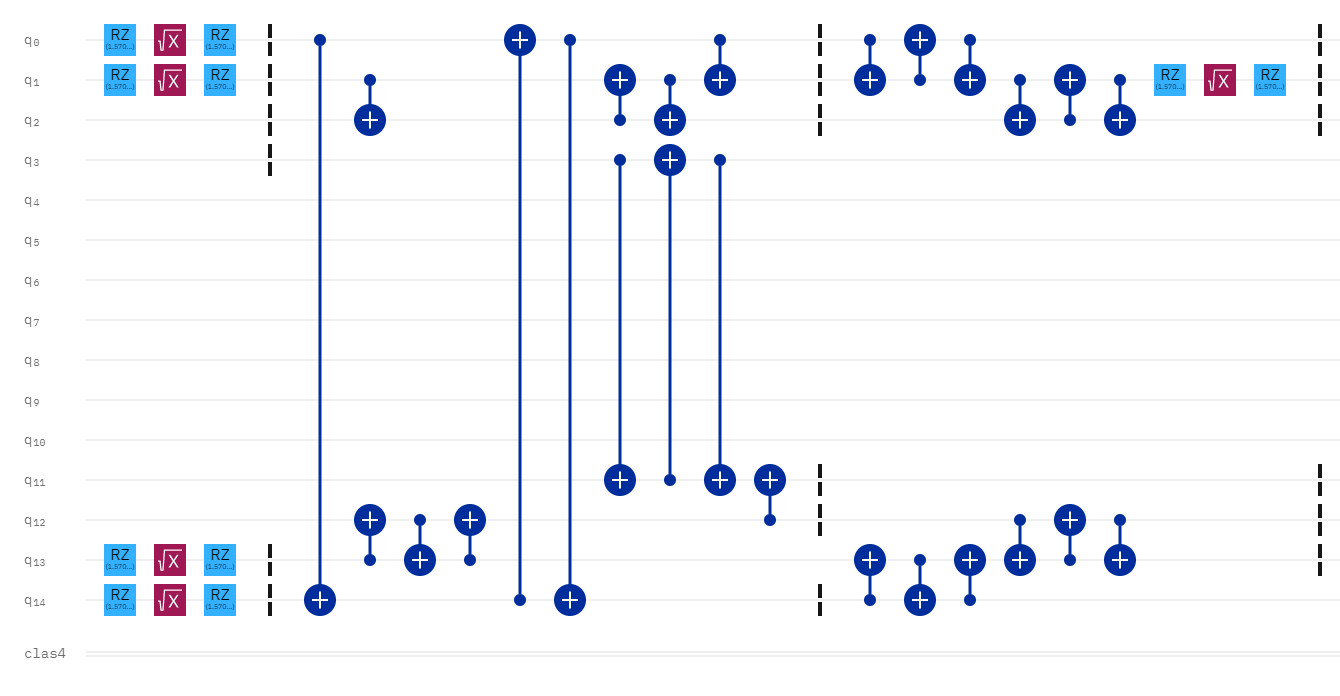
\includegraphics[width = 0.9\linewidth]{figures/transpiled_i.png}
    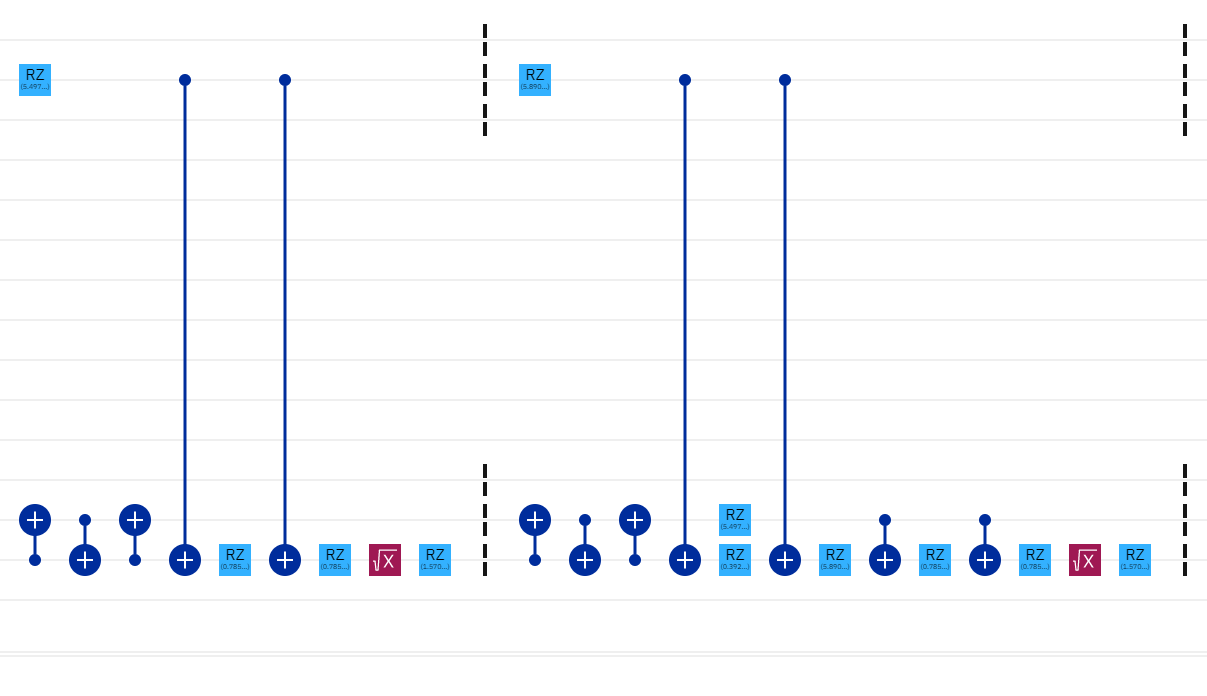
\includegraphics[width = 0.9\linewidth]{figures/transpiled_ii.png}
    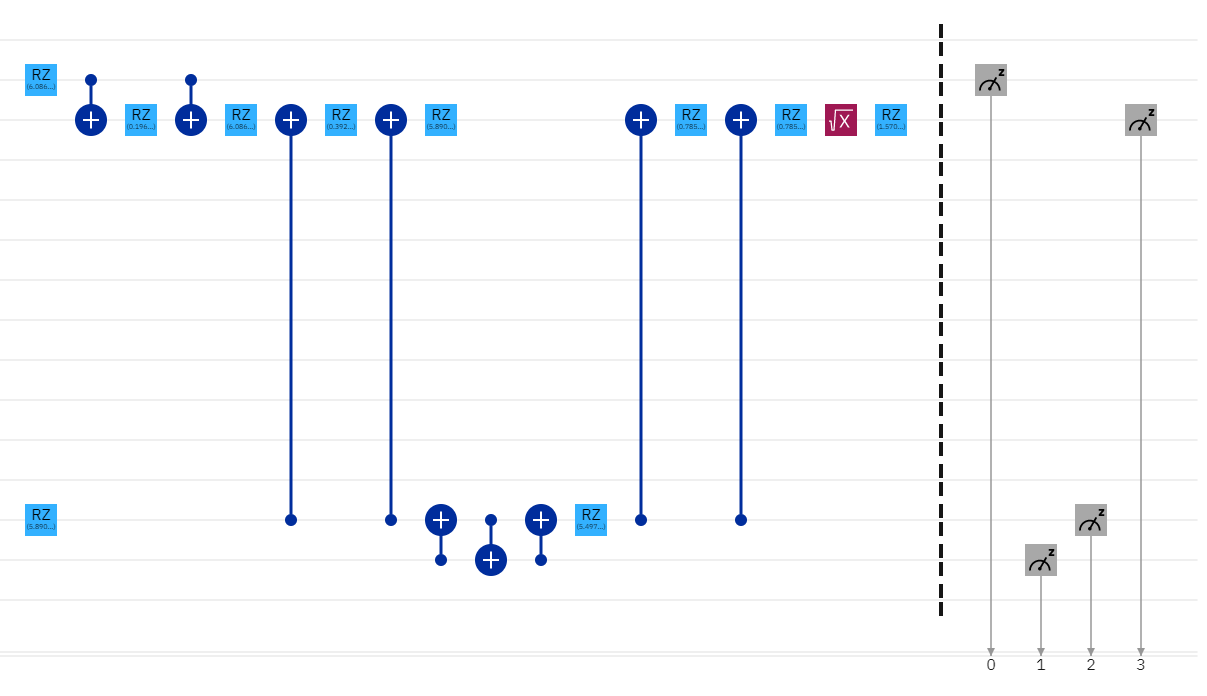
\includegraphics[width = 0.9\linewidth]{figures/transpiled_iii.png}
  \caption{Circuit Diagram of upon transpilation of original circuit(\ref{fig: Shor compiled circuit for fermat's prime})}
  \label{fig: Transpiled circuit diagram}
\end{figure}

